\documentclass[a4paper]{article}

\usepackage{INTERSPEECH2018}
\usepackage{tikz}
\usepackage{url}
\usepackage{blindtext}
\usetikzlibrary{shapes,arrows,positioning}

\tikzstyle{block} = [draw, fill=white, rectangle, 
    minimum height=3em, minimum width=6em]
\tikzstyle{sum} = [draw, fill=white, circle, node distance=1cm]
\tikzstyle{input} = [coordinate]
\tikzstyle{output} = [coordinate]
\tikzstyle{pinstyle} = [pin edge={to-,thin,black}]

\title{Multi-speaker articulatory-to-acoustic speech synthesis with
deep neural networks}
\name{Bence Halpern$^1$$^2$, Rob J. J. H. van Son$^1$, Michiel W. M.
  van den Brekel$^1$$^2$}
%The maximum number of authors in the author list is twenty. If the number of contributing authors is more than twenty, they should be listed in a footnote or in acknowledgement section, as appropriate.
\address{
  $^1$NKI-AVL, Amsterdam\\
  $^2$ACLC,University of Amsterdam, The Netherlands}
\email{b.halpern@nki.nl, r.v.son@nki.nl}

\begin{document}

\maketitle
% 
\begin{abstract}
  \blindtext[1]
\end{abstract}
\noindent\textbf{Index Terms}: computational paralinguistics, articulatory-to-acoustic
speech synthesis, deep learning, pathological speech

\section{Introduction}

Understading how articulation affects speech is a central question in speech
research. The source-filter model was one of the first models to tackle this
problem by noting that speech production could be described by
the geometry of the vocal tract and the glottal wave. Mathematically,
the model synthetises speech by exciting an autoregressive (AR) model with a
discrete time signal, where the AR coefficients capture the geometry of the
vocal tract, which is also represented by an area function \cite{Benesty2009}. 

\begin{figure}[t]
  \begin{center}
    \scalebox{0.75}{
  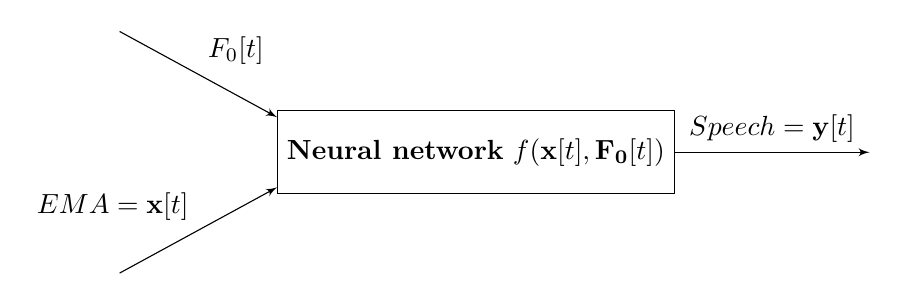
\begin{tikzpicture}[auto, node distance=5cm,>=latex']
    \node [input] (f0) {$F_0$};
  \node [block, below right = 1 cm and 2 cm of f0] (predictor) { \textbf{Neural network} $f(\mathbf{x}[t], \mathbf{F_0}[t]) $ };
  \node [input, name=input, right of = predictor] (speech) {Speech};
    \node [input, below left = 1 cm and 2 cm of predictor] (ema) {};
    \draw [->] (f0) -- node {$ F_0[t] $}   (predictor.170);
    \draw [->] (ema) -- node {$ \text{EMA} = \mathbf{x}[t] $}   (predictor.190);
    \draw [->] (predictor) -- node {$ \text{Speech} = \mathbf{y}[t] $} (speech);
  \end{tikzpicture}
}

    \scalebox{0.75}{
  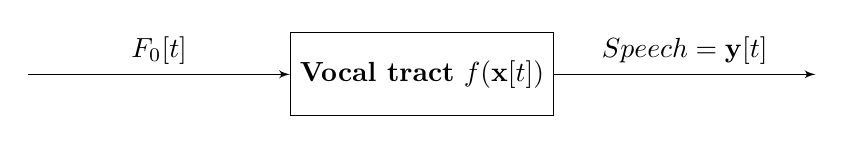
\begin{tikzpicture}[auto, node distance=5cm,>=latex']
    \node [input] (f0) {$F_0$};
  \node [block, right of = f0] (predictor) { \textbf{Vocal tract} $f(\mathbf{x}[t]) $ };
  \node [input, name=input, right of = predictor] (speech) {Speech};
    \draw [->] (f0) -- node {$ F_0[t] $}   (predictor);
    \draw [->] (predictor) -- node {$ \text{Speech} = \mathbf{y}[t] $} (speech);
  \end{tikzpicture}
 }
 \caption{Black box diagram showing the parallelities of a neural network
   based model with a source-filter model}
  \label{fig1}
    \end{center}
  \end{figure}

Recently, deep learning methods became popular
to understand articulation. These methods use a measurement tool,
called electromagnetic articulography to obtain articulation data 
\cite{Aryal2016} \cite{Taguchi} \cite{Liu2018} along with recurrent
neural networks, which are neural networks that are able to deal with
the sequential nature of data. Data-driven methods became of interest also
real-time speech synthesis. The efficacy of real-time speech synthesis
has been investigated using a tool called permanent magnetic articulography
by Gonzalez et al \cite{Gonzalez2017}, which gave understandable
speech.

The conclusion of these endeavours were that while it is possible to
predict some of the pitch from articulation, the quality of the speech
suffers. It was also possible to obtain satisfactory values for the
spectral quality.

In the author's broader research, the aim is to demonstrate how pathologies in
articulation are translated to speech. This of interest in many types
of pathological speech where the laryngeal functions remains intact, or
the deviations in the laryngeal function are known. This way accomodating
the articulatory changes to a model is able to aid understanding of
the pitch of the voice which has no pathological deviations.

Furthermore, based on the principles of the source-filter model,
it is then desirable to construct a data-driven method for
multi-speaker articulatory synthesis, which separates the source infomation
(excitation and articulation) from the effect (speech). 

The main contributions of this paper are,
\begin{itemize}
\item a set of benchmarks for multi-speaker articulatory to acoustic synthesis
\item estimation on how much data would be needed to construct a better model
\item an example of how to construct pathological speech using this framework
\end{itemize}

Our code is also available as a Github repository on the link
\url{https://github.com/karkirowle/vocoder-clean}.

\section{Method}
\subsection{Electromagnetic articulography}

Electromagnetic articulography uses sensor coils which are placed on the
different articulators in the vocal tract. Using this technology it
is possible to record the displacement of the articulators which can then
be used to approximate the dynamic area function with a neural network.

The electrodes are placed on the MNGU0 and MOCHA-TIMIT dataset on a total
of seven positions.
\begin{table}[th]
  \caption{Articulatory information recorded in datasets}
  \label{tab:example}
  \centering
  \begin{tabular}{ r r }
    \toprule
    \textbf{MNGU0} & \textbf{MOCHA-TIMIT} \\
    \midrule
    Tongue dorsum (T3) & Tongue dorsum (T3) \\
    Tongue blades (T2) & Tongue blades (T2) \\
    Tongue tip (T1) & Tongue tip (T1) \\
    Lower incisor (T3) & Jaw \\
    Upper incisor & Nose \\
    Upper lip & Upper lip \\
    Lower lip & Lower lip \\
    \bottomrule
  \end{tabular}
  
\end{table}

TODO: Decide whether you want to leave out the lower incisor or jaw
ii
\begin{figure}[t]
  \begin{center}
    \scalebox{0.50}{\input{init_pos.pgf}}
  \caption{The visualisation of electrode locations for all samples in
    the MNGU0 dataset at time point \( t = 0 \)}
\end{center}
\end{figure}
\subsection{Dataset}

The MNGU0 and the MOCHA-TIMIT dataset were used to obtain a total of
X samples, which were partitioned to training-validation set. The
combined dataset has 2274 speech recordings and electromagnetic articulography
data pairs. The dataset contains data from three speakers, two British
male and one British female.

\subsection{Preprocessing}

\subsection{Sampling}

It is important that the input and output sample rates of the different
datasets are matched, because otherwise, the input-output pairs contain
different amount of information.

The sampling frequency of the original EMA signals were 500 Hz, however
the MNGU0 was provided to us downsampled to 200 Hz. To match this frequency,
the sampling frequency of the MOCHA-TIMIT were also downsampled.

For the MNGU0 dataset, NaN values were of EMA occured, this was interpolated
linearly.

For the MOCHA-TIMIT dataset, a Savitzky-Golay filter was used to ...
(TODO: Savgol filter?)

To ease training, the input signals were either truncated or padded
so there were a total of \( T = 1000 \) samples for each training example.
For input signals which are shorter, it is assumed that the last part is
silence, so it is padded with the last element.

\subsection{Vocoder analysis}

The speech was transformed with the PyWORLD vocoder \cite{Morise2016}
and compressed with the PySPTK toolkit available at \url{http://github.com/r9y9/pysptk}.
The period between consecutive frames was 5 miliseconds. The resulting 40 MFCC and 1 power parameters
were used to generatic static and delta parameters, resulting in 82 parameters
for the training. As the first step of the MFCC processsing \( \alpha
= 0.42 \) were used a pre-emphasis coefficient. The PyWORLD vocoder
also provides the $ F_0 $ and BAP values for synthesis, these were
explicitly given for the synthesis.

\subsection{Delay and interpolation}
Previously \cite{Gonzalez2016}, the effect of delay on the
output signal were investigated. While it has been found that delay
is beneficial, the author's choice of function approximators are
restricted to acausal models, so it has been decided
not to use delay in our final implementation.

\subsection{Fundamental frequency}

Previously, it has been found beneficial to take the logarithm of the
pitch and linearly interpolate. \cite{Gonzalez2017} An alternative method also exists with
exponential interpolation which is described in \cite{Chen1997}.
It has been decided that the linear interpolation technique will be used.
This makes the \( F_0 \) continous, which is important property to have
when it is regressed in a function approximation setting.

\subsection{Normalisation}

Exploratory data analysis indicated that the articulatory trajectories of
the datasets were on different scale and bias, so it was normalised
on a per speaker basis. The output MFCCs were normalised for each cepstral
coefficients.

\subsection{Neural network}

To approximate the functional relationship, the authors have decided to
train a Bidirectional Long-Short Term Memory based neural network \cite{Hochreiter1997}. 

For all BLSTM layers, the CuDNNLSTM implementation have been used to
improve efficiency, however this limits the activation function to be
stricly \( \text{tanh}(\cdot) \)

A LSTM is governed by the following equations,

\begin{equation}
  \mathbf{i}_{t} = \sigma ( \mathbf{W}_{xi} \mathbf{x}_{t} + \mathbf{W}_{hi}
  \mathbf{h}_{t-1} + \mathbf{W}_{ci} \mathbf{c}_{t-1} + \mathbf{b}_{i})  
\end{equation}
\begin{equation}
  \mathbf{f}_{t} = \sigma ( \mathbf{W}_{xf} \mathbf{x}_{t} + \mathbf{W}_{hf}
  \mathbf{h}_{t-1} + \mathbf{W}_{cf} \mathbf{c}_{t-1} + \mathbf{b}_{f})  
\end{equation}
\begin{equation}
  \mathbf{c}_{t} = \mathbf{f} \mathbf{c}_{t-1} + \mathbf{i}_{t} \text{tanh} ( \mathbf{W}_{hc}
  \mathbf{h}_{t-1} + \mathbf{b}_c)
\end{equation}
\begin{equation}
  \mathbf{o}_{t} = \sigma ( \mathbf{W}_{x0}\mathbf{x}_t + \mathbf{W}_{ho} \mathbf{h}_{t-1}
  + \mathbf{W}_{co}\mathbf{c}_{t} + \mathbf{b}_0 )
\end{equation}
\begin{equation}
  \mathbf{h}_t = \mathbf{o}_{t} \text{tanh} ( \mathbf{c}_t )
  \end{equation}

\subsection{Synthesis}

A slighlty different method were undertaken for synthesis. It might
seem unconventional, that we don't predidict BAP and $ F_0 $, but $ F_0 $
is directly related to laryngeal function, so it is at the input side
of the actual speech synthesis.

\section{Experiment}

\subsection{Neural network experiments}

Three recurrent neural networks architectures were trained based on previous
papers tackling similiar problems.
aa
Based on \cite{Liu2018}, a bidirectional LSTM was trained with four layers.
The final layer was a fully connected layer matching the output dimensions.
This neural network was trained using stochastic gradient descent and
a learning rate of \( \alpha = 0.01 \).
ii
The ypublication of \cite{Taguchi} used a neural networks with...
This neural network was trained using RMSProp, with a learning rate of 0.01.

\begin{table}[th]
  \caption{Comparison of different trainng methods}
  \label{tab:example}
  \centering
  \begin{tabular}{ r r r }
    \toprule
    \textbf{Architecture} & \textbf{Optimiser} & \textbf{Base learning rate} \\
    \midrule
    Liu 2018 & SGD & 0.01 \\
    Taguchi 2018 & RMSProp & 0.01       \\
    Gonzalez 2017 & SGD (?) & 0.01               \\
    \bottomrule
  \end{tabular}
  
\end{table}

For training the mean squared error loss function was used, and for
evaluation the Mel cepstral distortion (MCD) have been employed. \cite{Kubichek1993}



Ten fold cross-validation was performed to estimate the out-ouf-sample
generalisation capability of the neural networks.

\subsection{Pathological speech synthesis}

Pathological speech synthesis is performed by considering the articulatory
space and taking knowledge about the change of articulation.

In tongue cancer, articulation of the tongue is impeded. In practice,
it is found that teaching patients to speak at a slower rate helps these
articulation problems. Thus, it is hypothesised that is the maximum
velocity of the tongue that is limited in pathological speech.

A pathological speech transformation could then be constructed for
a discretet time signal by first taking the discrete time difference,

\begin{equation}
  d[t] = x[t] - x[t-1],
  \label{eq1}
\end{equation}

where \( x[t] \in \mathbb{R}^T \) is a signal for one particular electrode channel.

The difference signal then can be thresholded using,

\begin{equation}
  d_p[t] = \text{min}(d[t],c) \quad \text{for} \quad d[t] \geq 0, 
  \label{eq2}
\end{equation}
\begin{equation}
  d_p[t] = \text{min}(d[t],-c) \quad \text{for} \quad d[t] < 0,
  \label{eq3}
\end{equation}

where \( c \in \mathbb{R}^{+} \) is a positive number representing an
arbitrary threshold.

After obtaining this signal a cumulative sum could be performed to obtain
the pathological EMA signal
\begin{equation}
  p[t] = \sum_{i=0}^{t} x[i].
  \label{eq4}
\end{equation}

This signal then could be fed through a feedforward run of a neural network
to synthetise pathological speech.

\section{Results and discussion}
\begin{table}[th]
  \caption{Comparison of 10-fold CV performance of neural networks}
  \label{tab:example}
  \centering
  \begin{tabular}{ r r }
    \toprule
    \textbf{Architecture} & \textbf{MCD} \\
    \midrule
    Liu 2018 & 5.8 dB \\
    Taguchi 2018 & 6.2 dB               \\
    Gonzalez 2017 & 6 dB               \\
    \bottomrule
  \end{tabular}
  
\end{table}

It is important to note that the original networks were trained on
single speakers, that is why the MCD values are higher than in the
original publications.

It can be concluded that it is possible to make satisfactory quality
speech synthesis, and it is possible to present some lisping pathologies.

\section{Conclusion}

\section{Acknowledgements}
This project has received funding from the European Union's Horizon
2020 research and innovation programme under Marie Sklodowska-Curie
grant agreement No 766287.



\bibliographystyle{IEEEtran}

\bibliography{paper1}


\end{document}
